\documentclass[1p]{elsarticle_modified}
%\bibliographystyle{elsarticle-num}

%\usepackage[colorlinks]{hyperref}
%\usepackage{abbrmath_seonhwa} %\Abb, \Ascr, \Acal ,\Abf, \Afrak
\usepackage{amsfonts}
\usepackage{amssymb}
\usepackage{amsmath}
\usepackage{amsthm}
\usepackage{scalefnt}
\usepackage{amsbsy}
\usepackage{kotex}
\usepackage{caption}
\usepackage{subfig}
\usepackage{color}
\usepackage{graphicx}
\usepackage{xcolor} %% white, black, red, green, blue, cyan, magenta, yellow
\usepackage{float}
\usepackage{setspace}
\usepackage{hyperref}

\usepackage{tikz}
\usetikzlibrary{arrows}

\usepackage{multirow}
\usepackage{array} % fixed length table
\usepackage{hhline}

%%%%%%%%%%%%%%%%%%%%%
\makeatletter
\renewcommand*\env@matrix[1][\arraystretch]{%
	\edef\arraystretch{#1}%
	\hskip -\arraycolsep
	\let\@ifnextchar\new@ifnextchar
	\array{*\c@MaxMatrixCols c}}
\makeatother %https://tex.stackexchange.com/questions/14071/how-can-i-increase-the-line-spacing-in-a-matrix
%%%%%%%%%%%%%%%

\usepackage[normalem]{ulem}

\newcommand{\msout}[1]{\ifmmode\text{\sout{\ensuremath{#1}}}\else\sout{#1}\fi}
%SOURCE: \msout is \stkout macro in https://tex.stackexchange.com/questions/20609/strikeout-in-math-mode

\newcommand{\cancel}[1]{
	\ifmmode
	{\color{red}\msout{#1}}
	\else
	{\color{red}\sout{#1}}
	\fi
}

\newcommand{\add}[1]{
	{\color{blue}\uwave{#1}}
}

\newcommand{\replace}[2]{
	\ifmmode
	{\color{red}\msout{#1}}{\color{blue}\uwave{#2}}
	\else
	{\color{red}\sout{#1}}{\color{blue}\uwave{#2}}
	\fi
}

\newcommand{\Sol}{\mathcal{S}} %segment
\newcommand{\D}{D} %diagram
\newcommand{\A}{\mathcal{A}} %arc


%%%%%%%%%%%%%%%%%%%%%%%%%%%%%5 test

\def\sl{\operatorname{\textup{SL}}(2,\Cbb)}
\def\psl{\operatorname{\textup{PSL}}(2,\Cbb)}
\def\quan{\mkern 1mu \triangleright \mkern 1mu}

\theoremstyle{definition}
\newtheorem{thm}{Theorem}[section]
\newtheorem{prop}[thm]{Proposition}
\newtheorem{lem}[thm]{Lemma}
\newtheorem{ques}[thm]{Question}
\newtheorem{cor}[thm]{Corollary}
\newtheorem{defn}[thm]{Definition}
\newtheorem{exam}[thm]{Example}
\newtheorem{rmk}[thm]{Remark}
\newtheorem{alg}[thm]{Algorithm}

\newcommand{\I}{\sqrt{-1}}
\begin{document}

%\begin{frontmatter}
%
%\title{Boundary parabolic representations of knots up to 8 crossings}
%
%%% Group authors per affiliation:
%\author{Yunhi Cho} 
%\address{Department of Mathematics, University of Seoul, Seoul, Korea}
%\ead{yhcho@uos.ac.kr}
%
%
%\author{Seonhwa Kim} %\fnref{s_kim}}
%\address{Center for Geometry and Physics, Institute for Basic Science, Pohang, 37673, Korea}
%\ead{ryeona17@ibs.re.kr}
%
%\author{Hyuk Kim}
%\address{Department of Mathematical Sciences, Seoul National University, Seoul 08826, Korea}
%\ead{hyukkim@snu.ac.kr}
%
%\author{Seokbeom Yoon}
%\address{Department of Mathematical Sciences, Seoul National University, Seoul, 08826,  Korea}
%\ead{sbyoon15@snu.ac.kr}
%
%\begin{abstract}
%We find all boundary parabolic representation of knots up to 8 crossings.
%
%\end{abstract}
%\begin{keyword}
%    \MSC[2010] 57M25 
%\end{keyword}
%
%\end{frontmatter}

%\linenumbers
%\tableofcontents
%
\newcommand\colored[1]{\textcolor{white}{\rule[-0.35ex]{0.8em}{1.4ex}}\kern-0.8em\color{red} #1}%
%\newcommand\colored[1]{\textcolor{white}{ #1}\kern-2.17ex	\textcolor{white}{ #1}\kern-1.81ex	\textcolor{white}{ #1}\kern-2.15ex\color{red}#1	}

{\Large $\underline{12n_{0250}~(K12n_{0250})}$}

\setlength{\tabcolsep}{10pt}
\renewcommand{\arraystretch}{1.6}
\vspace{1cm}\begin{tabular}{m{100pt}>{\centering\arraybackslash}m{274pt}}
\multirow{5}{120pt}{
	\centering
	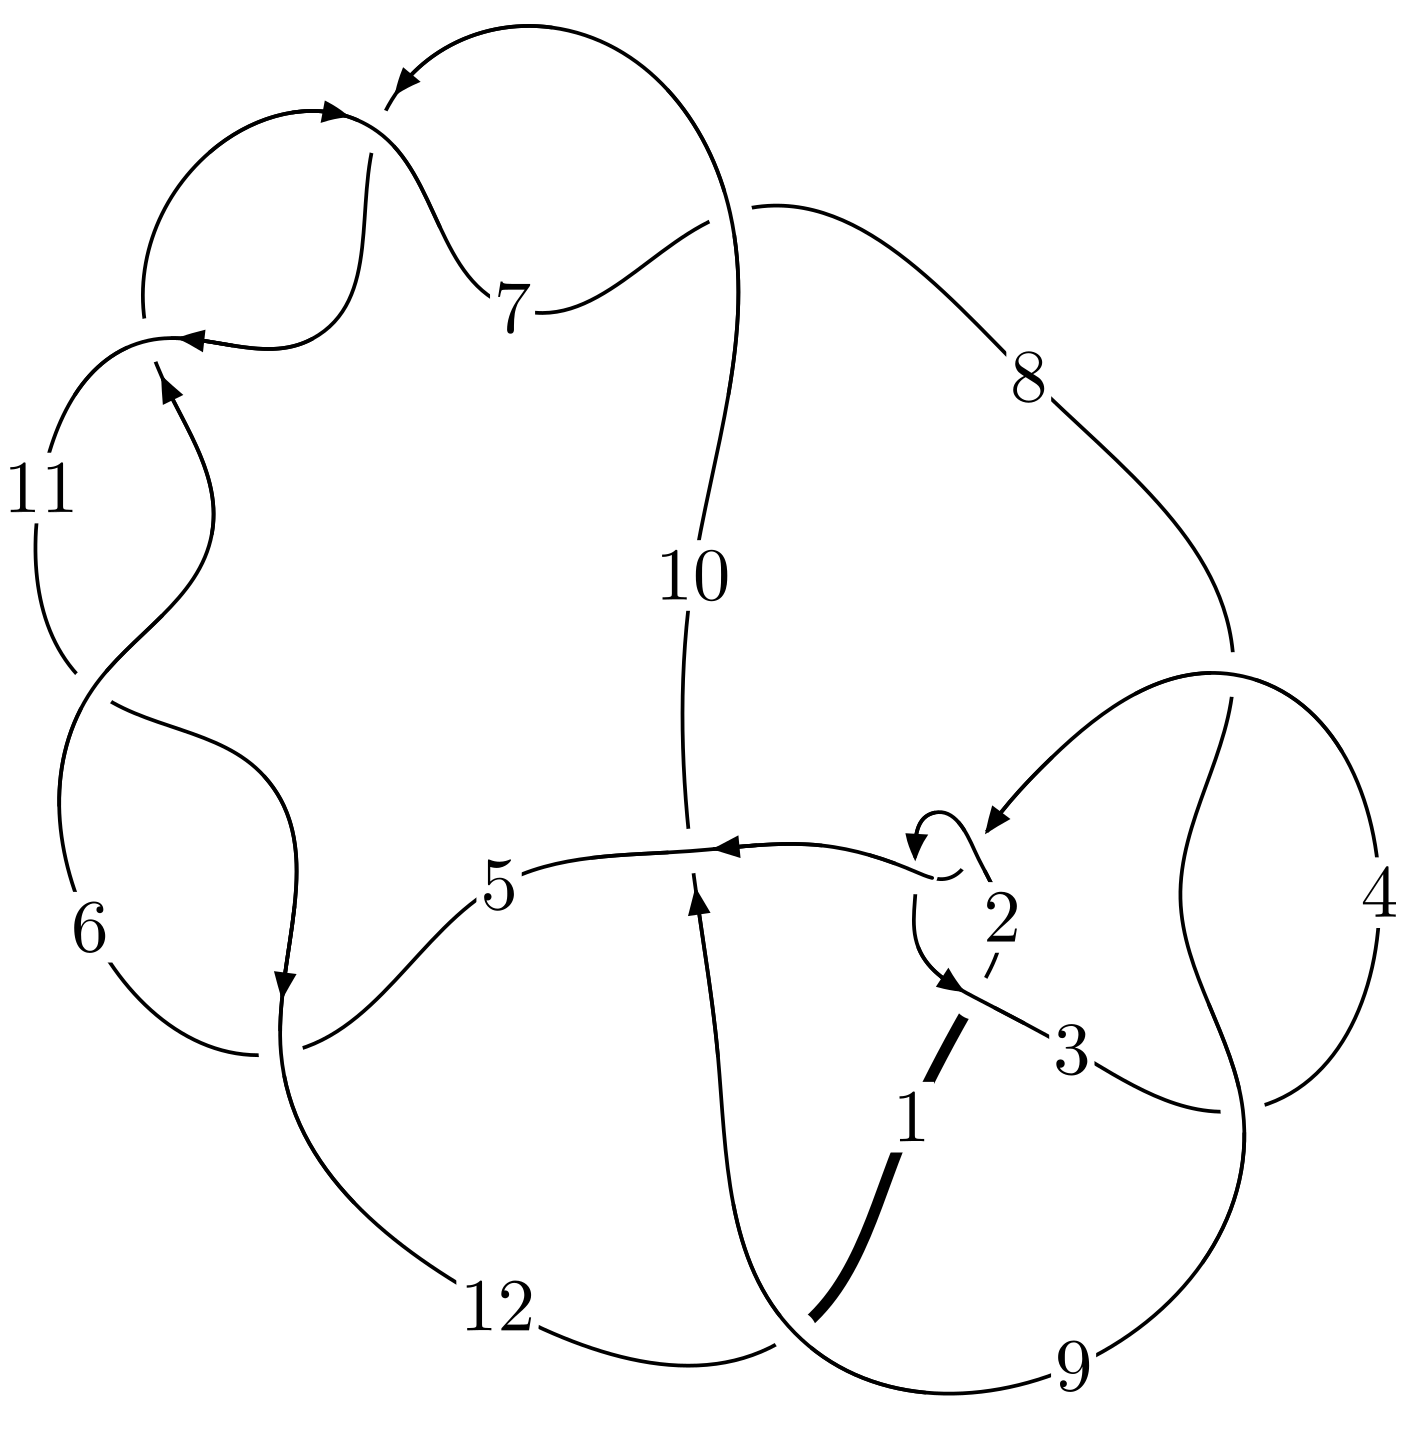
\includegraphics[width=112pt]{../../../GIT/diagram.site/Diagrams/png/2339_12n_0250.png}\\
\ \ \ A knot diagram\footnotemark}&
\allowdisplaybreaks
\textbf{Linearized knot diagam} \\
\cline{2-2}
 &
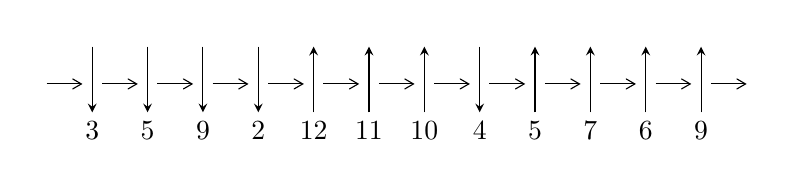
\begin{tikzpicture}[x=20pt, y=17pt]
	% nodes
	\node (C0) at (0, 0) {};
	\node (C1) at (1, 0) {};
	\node (C1U) at (1, +1) {};
	\node (C1D) at (1, -1) {3};

	\node (C2) at (2, 0) {};
	\node (C2U) at (2, +1) {};
	\node (C2D) at (2, -1) {5};

	\node (C3) at (3, 0) {};
	\node (C3U) at (3, +1) {};
	\node (C3D) at (3, -1) {9};

	\node (C4) at (4, 0) {};
	\node (C4U) at (4, +1) {};
	\node (C4D) at (4, -1) {2};

	\node (C5) at (5, 0) {};
	\node (C5U) at (5, +1) {};
	\node (C5D) at (5, -1) {12};

	\node (C6) at (6, 0) {};
	\node (C6U) at (6, +1) {};
	\node (C6D) at (6, -1) {11};

	\node (C7) at (7, 0) {};
	\node (C7U) at (7, +1) {};
	\node (C7D) at (7, -1) {10};

	\node (C8) at (8, 0) {};
	\node (C8U) at (8, +1) {};
	\node (C8D) at (8, -1) {4};

	\node (C9) at (9, 0) {};
	\node (C9U) at (9, +1) {};
	\node (C9D) at (9, -1) {5};

	\node (C10) at (10, 0) {};
	\node (C10U) at (10, +1) {};
	\node (C10D) at (10, -1) {7};

	\node (C11) at (11, 0) {};
	\node (C11U) at (11, +1) {};
	\node (C11D) at (11, -1) {6};

	\node (C12) at (12, 0) {};
	\node (C12U) at (12, +1) {};
	\node (C12D) at (12, -1) {9};
	\node (C13) at (13, 0) {};

	% arrows
	\draw[->,>={angle 60}]
	(C0) edge (C1) (C1) edge (C2) (C2) edge (C3) (C3) edge (C4) (C4) edge (C5) (C5) edge (C6) (C6) edge (C7) (C7) edge (C8) (C8) edge (C9) (C9) edge (C10) (C10) edge (C11) (C11) edge (C12) (C12) edge (C13) ;	\draw[->,>=stealth]
	(C1U) edge (C1D) (C2U) edge (C2D) (C3U) edge (C3D) (C4U) edge (C4D) (C5D) edge (C5U) (C6D) edge (C6U) (C7D) edge (C7U) (C8U) edge (C8D) (C9D) edge (C9U) (C10D) edge (C10U) (C11D) edge (C11U) (C12D) edge (C12U) ;
	\end{tikzpicture} \\
\hhline{~~} \\& 
\textbf{Solving Sequence} \\ \cline{2-2} 
 &
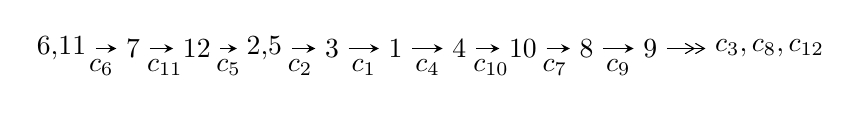
\begin{tikzpicture}[x=23pt, y=7pt]
	% node
	\node (A0) at (-1/8, 0) {6,11};
	\node (A1) at (1, 0) {7};
	\node (A2) at (2, 0) {12};
	\node (A3) at (49/16, 0) {2,5};
	\node (A4) at (33/8, 0) {3};
	\node (A5) at (41/8, 0) {1};
	\node (A6) at (49/8, 0) {4};
	\node (A7) at (57/8, 0) {10};
	\node (A8) at (65/8, 0) {8};
	\node (A9) at (73/8, 0) {9};
	\node (C1) at (1/2, -1) {$c_{6}$};
	\node (C2) at (3/2, -1) {$c_{11}$};
	\node (C3) at (5/2, -1) {$c_{5}$};
	\node (C4) at (29/8, -1) {$c_{2}$};
	\node (C5) at (37/8, -1) {$c_{1}$};
	\node (C6) at (45/8, -1) {$c_{4}$};
	\node (C7) at (53/8, -1) {$c_{10}$};
	\node (C8) at (61/8, -1) {$c_{7}$};
	\node (C9) at (69/8, -1) {$c_{9}$};
	\node (A10) at (11, 0) {$c_{3},c_{8},c_{12}$};

	% edge
	\draw[->,>=stealth]	
	(A0) edge (A1) (A1) edge (A2) (A2) edge (A3) (A3) edge (A4) (A4) edge (A5) (A5) edge (A6) (A6) edge (A7) (A7) edge (A8) (A8) edge (A9) ;
	\draw[->>,>={angle 60}]	
	(A9) edge (A10);
\end{tikzpicture} \\ 

\end{tabular} \\

\footnotetext{
The image of knot diagram is generated by the software ``\textbf{Draw programme}" developed by Andrew Bartholomew(\url{http://www.layer8.co.uk/maths/draw/index.htm\#Running-draw}), where we modified some parts for our purpose(\url{https://github.com/CATsTAILs/LinksPainter}).
}\phantom \\ \newline 
\centering \textbf{Ideals for irreducible components\footnotemark of $X_{\text{par}}$} 
 
\begin{align*}
I^u_{1}&=\langle 
u^{21}-2 u^{20}+\cdots+b-1,\;u^{24}-2 u^{23}+\cdots+a+3,\;u^{25}-2 u^{24}+\cdots+5 u-1\rangle \\
I^u_{2}&=\langle 
u^2+b+u+1,\;- u^4- u^3-3 u^2+a-2 u-1,\;u^5+u^4+4 u^3+3 u^2+3 u+1\rangle \\
\\
\end{align*}
\raggedright * 2 irreducible components of $\dim_{\mathbb{C}}=0$, with total 30 representations.\\
\footnotetext{All coefficients of polynomials are rational numbers. But the coefficients are sometimes approximated in decimal forms when there is not enough margin.}
\newpage
\renewcommand{\arraystretch}{1}
\centering \section*{I. $I^u_{1}= \langle u^{21}-2 u^{20}+\cdots+b-1,\;u^{24}-2 u^{23}+\cdots+a+3,\;u^{25}-2 u^{24}+\cdots+5 u-1 \rangle$}
\flushleft \textbf{(i) Arc colorings}\\
\begin{tabular}{m{7pt} m{180pt} m{7pt} m{180pt} }
\flushright $a_{6}=$&$\begin{pmatrix}1\\0\end{pmatrix}$ \\
\flushright $a_{11}=$&$\begin{pmatrix}0\\u\end{pmatrix}$ \\
\flushright $a_{7}=$&$\begin{pmatrix}1\\- u^2\end{pmatrix}$ \\
\flushright $a_{12}=$&$\begin{pmatrix}u\\u\end{pmatrix}$ \\
\flushright $a_{2}=$&$\begin{pmatrix}- u^{24}+2 u^{23}+\cdots+2 u-3\\- u^{21}+2 u^{20}+\cdots- u+1\end{pmatrix}$ \\
\flushright $a_{5}=$&$\begin{pmatrix}u^2+1\\u^2\end{pmatrix}$ \\
\flushright $a_{3}=$&$\begin{pmatrix}- u^{24}+2 u^{23}+\cdots+2 u-4\\- u^{22}-11 u^{20}+\cdots- u+1\end{pmatrix}$ \\
\flushright $a_{1}=$&$\begin{pmatrix}u^{13}+8 u^{11}+23 u^9+30 u^7+20 u^5+6 u^3+u\\u^{13}+7 u^{11}+15 u^9+8 u^7-4 u^5-3 u^3+u\end{pmatrix}$ \\
\flushright $a_{4}=$&$\begin{pmatrix}u^{24}-2 u^{23}+\cdots+u+3\\- u^{22}+2 u^{21}+\cdots+2 u-1\end{pmatrix}$ \\
\flushright $a_{10}=$&$\begin{pmatrix}- u\\u^3+u\end{pmatrix}$ \\
\flushright $a_{8}=$&$\begin{pmatrix}u^2+1\\- u^4-2 u^2\end{pmatrix}$ \\
\flushright $a_{9}=$&$\begin{pmatrix}- u^7-4 u^5-4 u^3-2 u\\- u^7-3 u^5+u\end{pmatrix}$\\&\end{tabular}
\flushleft \textbf{(ii) Obstruction class $= -1$}\\~\\
\flushleft \textbf{(iii) Cusp Shapes $= - u^{24}+2 u^{23}-18 u^{22}+32 u^{21}-142 u^{20}+222 u^{19}-644 u^{18}+875 u^{17}-1848 u^{16}+2155 u^{15}-3472 u^{14}+3429 u^{13}-4258 u^{12}+3506 u^{11}-3270 u^{10}+2195 u^9-1387 u^8+732 u^7-164 u^6+62 u^5+90 u^4-28 u^3+16 u^2-3 u-10$}\\~\\
\newpage\renewcommand{\arraystretch}{1}
\flushleft \textbf{(iv) u-Polynomials at the component}\newline \\
\begin{tabular}{m{50pt}|m{274pt}}
Crossings & \hspace{64pt}u-Polynomials at each crossing \\
\hline $$\begin{aligned}c_{1}\end{aligned}$$&$\begin{aligned}
&u^{25}+4 u^{24}+\cdots-5 u+1
\end{aligned}$\\
\hline $$\begin{aligned}c_{2},c_{4}\end{aligned}$$&$\begin{aligned}
&u^{25}-6 u^{24}+\cdots-5 u+1
\end{aligned}$\\
\hline $$\begin{aligned}c_{3},c_{8}\end{aligned}$$&$\begin{aligned}
&u^{25}- u^{24}+\cdots+32 u+32
\end{aligned}$\\
\hline $$\begin{aligned}c_{5},c_{6},c_{7}\\c_{10},c_{11}\end{aligned}$$&$\begin{aligned}
&u^{25}+2 u^{24}+\cdots+5 u+1
\end{aligned}$\\
\hline $$\begin{aligned}c_{9}\end{aligned}$$&$\begin{aligned}
&u^{25}+2 u^{24}+\cdots+3 u+1
\end{aligned}$\\
\hline $$\begin{aligned}c_{12}\end{aligned}$$&$\begin{aligned}
&u^{25}-8 u^{24}+\cdots+14437 u-1751
\end{aligned}$\\
\hline
\end{tabular}\\~\\
\newpage\renewcommand{\arraystretch}{1}
\flushleft \textbf{(v) Riley Polynomials at the component}\newline \\
\begin{tabular}{m{50pt}|m{274pt}}
Crossings & \hspace{64pt}Riley Polynomials at each crossing \\
\hline $$\begin{aligned}c_{1}\end{aligned}$$&$\begin{aligned}
&y^{25}+40 y^{24}+\cdots-5 y-1
\end{aligned}$\\
\hline $$\begin{aligned}c_{2},c_{4}\end{aligned}$$&$\begin{aligned}
&y^{25}-4 y^{24}+\cdots-5 y-1
\end{aligned}$\\
\hline $$\begin{aligned}c_{3},c_{8}\end{aligned}$$&$\begin{aligned}
&y^{25}+33 y^{24}+\cdots-3584 y-1024
\end{aligned}$\\
\hline $$\begin{aligned}c_{5},c_{6},c_{7}\\c_{10},c_{11}\end{aligned}$$&$\begin{aligned}
&y^{25}+32 y^{24}+\cdots+25 y-1
\end{aligned}$\\
\hline $$\begin{aligned}c_{9}\end{aligned}$$&$\begin{aligned}
&y^{25}-32 y^{24}+\cdots+25 y-1
\end{aligned}$\\
\hline $$\begin{aligned}c_{12}\end{aligned}$$&$\begin{aligned}
&y^{25}-44 y^{24}+\cdots+245499141 y-3066001
\end{aligned}$\\
\hline
\end{tabular}\\~\\
\newpage\flushleft \textbf{(vi) Complex Volumes and Cusp Shapes}
$$\begin{array}{c|c|c}  
\text{Solutions to }I^u_{1}& \I (\text{vol} + \sqrt{-1}CS) & \text{Cusp shape}\\
 \hline 
\begin{aligned}
u &= \phantom{-}0.459758 + 0.889622 I \\
a &= \phantom{-}0.076243 - 0.510379 I \\
b &= \phantom{-}0.96095 + 1.37863 I\end{aligned}
 & \phantom{-}7.04309 + 7.69753 I & \phantom{-}0.69223 - 5.87020 I \\ \hline\begin{aligned}
u &= \phantom{-}0.459758 - 0.889622 I \\
a &= \phantom{-}0.076243 + 0.510379 I \\
b &= \phantom{-}0.96095 - 1.37863 I\end{aligned}
 & \phantom{-}7.04309 - 7.69753 I & \phantom{-}0.69223 + 5.87020 I \\ \hline\begin{aligned}
u &= -0.233597 + 0.958426 I \\
a &= -0.400131 + 0.212647 I \\
b &= \phantom{-}0.719444 - 0.275653 I\end{aligned}
 & -2.25524 - 2.86318 I & \phantom{-}0.67832 + 5.18628 I \\ \hline\begin{aligned}
u &= -0.233597 - 0.958426 I \\
a &= -0.400131 - 0.212647 I \\
b &= \phantom{-}0.719444 + 0.275653 I\end{aligned}
 & -2.25524 + 2.86318 I & \phantom{-}0.67832 - 5.18628 I \\ \hline\begin{aligned}
u &= \phantom{-}0.480913 + 0.815098 I \\
a &= -0.540781 - 0.132936 I \\
b &= -1.59979 - 0.36621 I\end{aligned}
 & \phantom{-}7.50954 + 0.03310 I & \phantom{-}1.50006 - 1.57887 I \\ \hline\begin{aligned}
u &= \phantom{-}0.480913 - 0.815098 I \\
a &= -0.540781 + 0.132936 I \\
b &= -1.59979 + 0.36621 I\end{aligned}
 & \phantom{-}7.50954 - 0.03310 I & \phantom{-}1.50006 + 1.57887 I \\ \hline\begin{aligned}
u &= -0.277299 + 0.715967 I \\
a &= -0.206006 + 0.120919 I \\
b &= -0.106133 + 1.044080 I\end{aligned}
 & -0.57147 - 2.01138 I & \phantom{-}1.23672 + 5.35998 I \\ \hline\begin{aligned}
u &= -0.277299 - 0.715967 I \\
a &= -0.206006 - 0.120919 I \\
b &= -0.106133 - 1.044080 I\end{aligned}
 & -0.57147 + 2.01138 I & \phantom{-}1.23672 - 5.35998 I \\ \hline\begin{aligned}
u &= \phantom{-}0.085005 + 0.759627 I \\
a &= \phantom{-}1.31404 + 0.60640 I \\
b &= \phantom{-}0.296392 - 1.022520 I\end{aligned}
 & -3.36592 + 0.96368 I & -4.01560 + 0.59686 I \\ \hline\begin{aligned}
u &= \phantom{-}0.085005 - 0.759627 I \\
a &= \phantom{-}1.31404 - 0.60640 I \\
b &= \phantom{-}0.296392 + 1.022520 I\end{aligned}
 & -3.36592 - 0.96368 I & -4.01560 - 0.59686 I\\
 \hline 
 \end{array}$$\newpage$$\begin{array}{c|c|c}  
\text{Solutions to }I^u_{1}& \I (\text{vol} + \sqrt{-1}CS) & \text{Cusp shape}\\
 \hline 
\begin{aligned}
u &= \phantom{-}0.683438 + 0.037064 I \\
a &= \phantom{-}0.47321 - 1.98307 I \\
b &= -0.484746 + 0.125338 I\end{aligned}
 & \phantom{-}9.85760 + 3.86250 I & \phantom{-}4.92075 - 2.49747 I \\ \hline\begin{aligned}
u &= \phantom{-}0.683438 - 0.037064 I \\
a &= \phantom{-}0.47321 + 1.98307 I \\
b &= -0.484746 - 0.125338 I\end{aligned}
 & \phantom{-}9.85760 - 3.86250 I & \phantom{-}4.92075 + 2.49747 I \\ \hline\begin{aligned}
u &= -0.454087 + 0.131996 I \\
a &= -0.930347 + 0.905066 I \\
b &= -0.170032 - 0.148405 I\end{aligned}
 & \phantom{-}1.125730 - 0.539778 I & \phantom{-}7.59664 + 2.57696 I \\ \hline\begin{aligned}
u &= -0.454087 - 0.131996 I \\
a &= -0.930347 - 0.905066 I \\
b &= -0.170032 + 0.148405 I\end{aligned}
 & \phantom{-}1.125730 + 0.539778 I & \phantom{-}7.59664 - 2.57696 I \\ \hline\begin{aligned}
u &= -0.05917 + 1.63615 I \\
a &= \phantom{-}0.26489 + 2.09173 I \\
b &= \phantom{-}0.28511 + 2.85242 I\end{aligned}
 & -8.78516 - 3.17139 I & -0.87361 + 3.19607 I \\ \hline\begin{aligned}
u &= -0.05917 - 1.63615 I \\
a &= \phantom{-}0.26489 - 2.09173 I \\
b &= \phantom{-}0.28511 - 2.85242 I\end{aligned}
 & -8.78516 + 3.17139 I & -0.87361 - 3.19607 I \\ \hline\begin{aligned}
u &= \phantom{-}0.12897 + 1.64332 I \\
a &= -1.43354 - 1.14853 I \\
b &= -1.74726 - 1.22919 I\end{aligned}
 & -0.90994 + 2.33809 I & -0.195140 - 0.570968 I \\ \hline\begin{aligned}
u &= \phantom{-}0.12897 - 1.64332 I \\
a &= -1.43354 + 1.14853 I \\
b &= -1.74726 + 1.22919 I\end{aligned}
 & -0.90994 - 2.33809 I & -0.195140 + 0.570968 I \\ \hline\begin{aligned}
u &= \phantom{-}0.01776 + 1.65047 I \\
a &= -0.47939 - 1.88937 I \\
b &= -1.43279 - 2.83187 I\end{aligned}
 & -11.86300 + 1.31883 I & -3.44425 + 0. I\phantom{ +0.000000I} \\ \hline\begin{aligned}
u &= \phantom{-}0.01776 - 1.65047 I \\
a &= -0.47939 + 1.88937 I \\
b &= -1.43279 + 2.83187 I\end{aligned}
 & -11.86300 - 1.31883 I & -3.44425 + 0. I\phantom{ +0.000000I}\\
 \hline 
 \end{array}$$\newpage$$\begin{array}{c|c|c}  
\text{Solutions to }I^u_{1}& \I (\text{vol} + \sqrt{-1}CS) & \text{Cusp shape}\\
 \hline 
\begin{aligned}
u &= \phantom{-}0.12689 + 1.67737 I \\
a &= \phantom{-}1.19016 + 2.59619 I \\
b &= \phantom{-}2.22016 + 3.74930 I\end{aligned}
 & -1.85042 + 9.98114 I & -1.18698 - 4.78469 I \\ \hline\begin{aligned}
u &= \phantom{-}0.12689 - 1.67737 I \\
a &= \phantom{-}1.19016 - 2.59619 I \\
b &= \phantom{-}2.22016 - 3.74930 I\end{aligned}
 & -1.85042 - 9.98114 I & -1.18698 + 4.78469 I \\ \hline\begin{aligned}
u &= -0.05535 + 1.70735 I \\
a &= \phantom{-}1.56322 - 0.66579 I \\
b &= \phantom{-}2.67420 - 0.95840 I\end{aligned}
 & -11.72920 - 3.98033 I & \phantom{-0.000000 -}0. + 4.58718 I \\ \hline\begin{aligned}
u &= -0.05535 - 1.70735 I \\
a &= \phantom{-}1.56322 + 0.66579 I \\
b &= \phantom{-}2.67420 + 0.95840 I\end{aligned}
 & -11.72920 + 3.98033 I & \phantom{-0.000000 } 0. - 4.58718 I \\ \hline\begin{aligned}
u &= \phantom{-}0.193537\phantom{ +0.000000I} \\
a &= -2.78315\phantom{ +0.000000I} \\
b &= \phantom{-}0.768975\phantom{ +0.000000I}\end{aligned}
 & -1.31003\phantom{ +0.000000I} & -10.0440\phantom{ +0.000000I}\\
 \hline 
 \end{array}$$\newpage\newpage\renewcommand{\arraystretch}{1}
\centering \section*{II. $I^u_{2}= \langle u^2+b+u+1,\;- u^4- u^3-3 u^2+a-2 u-1,\;u^5+u^4+4 u^3+3 u^2+3 u+1 \rangle$}
\flushleft \textbf{(i) Arc colorings}\\
\begin{tabular}{m{7pt} m{180pt} m{7pt} m{180pt} }
\flushright $a_{6}=$&$\begin{pmatrix}1\\0\end{pmatrix}$ \\
\flushright $a_{11}=$&$\begin{pmatrix}0\\u\end{pmatrix}$ \\
\flushright $a_{7}=$&$\begin{pmatrix}1\\- u^2\end{pmatrix}$ \\
\flushright $a_{12}=$&$\begin{pmatrix}u\\u\end{pmatrix}$ \\
\flushright $a_{2}=$&$\begin{pmatrix}u^4+u^3+3 u^2+2 u+1\\- u^2- u-1\end{pmatrix}$ \\
\flushright $a_{5}=$&$\begin{pmatrix}u^2+1\\u^2\end{pmatrix}$ \\
\flushright $a_{3}=$&$\begin{pmatrix}u^4+u^3+4 u^2+2 u+2\\- u-1\end{pmatrix}$ \\
\flushright $a_{1}=$&$\begin{pmatrix}- u^2-1\\- u^2\end{pmatrix}$ \\
\flushright $a_{4}=$&$\begin{pmatrix}u^4+u^3+4 u^2+2 u+2\\- u-1\end{pmatrix}$ \\
\flushright $a_{10}=$&$\begin{pmatrix}- u\\u^3+u\end{pmatrix}$ \\
\flushright $a_{8}=$&$\begin{pmatrix}u^2+1\\- u^4-2 u^2\end{pmatrix}$ \\
\flushright $a_{9}=$&$\begin{pmatrix}u^2+1\\- u^4-2 u^2\end{pmatrix}$\\&\end{tabular}
\flushleft \textbf{(ii) Obstruction class $= 1$}\\~\\
\flushleft \textbf{(iii) Cusp Shapes $= 5 u^4+5 u^3+20 u^2+14 u+9$}\\~\\
\newpage\renewcommand{\arraystretch}{1}
\flushleft \textbf{(iv) u-Polynomials at the component}\newline \\
\begin{tabular}{m{50pt}|m{274pt}}
Crossings & \hspace{64pt}u-Polynomials at each crossing \\
\hline $$\begin{aligned}c_{1},c_{2}\end{aligned}$$&$\begin{aligned}
&(u-1)^5
\end{aligned}$\\
\hline $$\begin{aligned}c_{3},c_{8}\end{aligned}$$&$\begin{aligned}
&u^5
\end{aligned}$\\
\hline $$\begin{aligned}c_{4}\end{aligned}$$&$\begin{aligned}
&(u+1)^5
\end{aligned}$\\
\hline $$\begin{aligned}c_{5},c_{6},c_{7}\end{aligned}$$&$\begin{aligned}
&u^5+u^4+4 u^3+3 u^2+3 u+1
\end{aligned}$\\
\hline $$\begin{aligned}c_{9},c_{12}\end{aligned}$$&$\begin{aligned}
&u^5- u^4+u^2+u-1
\end{aligned}$\\
\hline $$\begin{aligned}c_{10},c_{11}\end{aligned}$$&$\begin{aligned}
&u^5- u^4+4 u^3-3 u^2+3 u-1
\end{aligned}$\\
\hline
\end{tabular}\\~\\
\newpage\renewcommand{\arraystretch}{1}
\flushleft \textbf{(v) Riley Polynomials at the component}\newline \\
\begin{tabular}{m{50pt}|m{274pt}}
Crossings & \hspace{64pt}Riley Polynomials at each crossing \\
\hline $$\begin{aligned}c_{1},c_{2},c_{4}\end{aligned}$$&$\begin{aligned}
&(y-1)^5
\end{aligned}$\\
\hline $$\begin{aligned}c_{3},c_{8}\end{aligned}$$&$\begin{aligned}
&y^5
\end{aligned}$\\
\hline $$\begin{aligned}c_{5},c_{6},c_{7}\\c_{10},c_{11}\end{aligned}$$&$\begin{aligned}
&y^5+7 y^4+16 y^3+13 y^2+3 y-1
\end{aligned}$\\
\hline $$\begin{aligned}c_{9},c_{12}\end{aligned}$$&$\begin{aligned}
&y^5- y^4+4 y^3-3 y^2+3 y-1
\end{aligned}$\\
\hline
\end{tabular}\\~\\
\newpage\flushleft \textbf{(vi) Complex Volumes and Cusp Shapes}
$$\begin{array}{c|c|c}  
\text{Solutions to }I^u_{2}& \I (\text{vol} + \sqrt{-1}CS) & \text{Cusp shape}\\
 \hline 
\begin{aligned}
u &= -0.233677 + 0.885557 I \\
a &= -0.758138 + 0.584034 I \\
b &= -0.036717 - 0.471689 I\end{aligned}
 & -3.46474 - 2.21397 I & -4.37343 + 4.39306 I \\ \hline\begin{aligned}
u &= -0.233677 - 0.885557 I \\
a &= -0.758138 - 0.584034 I \\
b &= -0.036717 + 0.471689 I\end{aligned}
 & -3.46474 + 2.21397 I & -4.37343 - 4.39306 I \\ \hline\begin{aligned}
u &= -0.416284\phantom{ +0.000000I} \\
a &= \phantom{-}0.645200\phantom{ +0.000000I} \\
b &= -0.757008\phantom{ +0.000000I}\end{aligned}
 & -0.762751\phantom{ +0.000000I} & \phantom{-}6.42730\phantom{ +0.000000I} \\ \hline\begin{aligned}
u &= -0.05818 + 1.69128 I \\
a &= \phantom{-}0.935538 - 0.903908 I \\
b &= \phantom{-}1.91522 - 1.49448 I\end{aligned}
 & -12.60320 - 3.33174 I & -5.84024 + 1.26157 I \\ \hline\begin{aligned}
u &= -0.05818 - 1.69128 I \\
a &= \phantom{-}0.935538 + 0.903908 I \\
b &= \phantom{-}1.91522 + 1.49448 I\end{aligned}
 & -12.60320 + 3.33174 I & -5.84024 - 1.26157 I\\
 \hline 
 \end{array}$$\newpage
\newpage\renewcommand{\arraystretch}{1}
\centering \section*{ III. u-Polynomials}
\begin{tabular}{m{50pt}|m{274pt}}
Crossings & \hspace{64pt}u-Polynomials at each crossing \\
\hline $$\begin{aligned}c_{1}\end{aligned}$$&$\begin{aligned}
&((u-1)^5)(u^{25}+4 u^{24}+\cdots-5 u+1)
\end{aligned}$\\
\hline $$\begin{aligned}c_{2}\end{aligned}$$&$\begin{aligned}
&((u-1)^5)(u^{25}-6 u^{24}+\cdots-5 u+1)
\end{aligned}$\\
\hline $$\begin{aligned}c_{3},c_{8}\end{aligned}$$&$\begin{aligned}
&u^5(u^{25}- u^{24}+\cdots+32 u+32)
\end{aligned}$\\
\hline $$\begin{aligned}c_{4}\end{aligned}$$&$\begin{aligned}
&((u+1)^5)(u^{25}-6 u^{24}+\cdots-5 u+1)
\end{aligned}$\\
\hline $$\begin{aligned}c_{5},c_{6},c_{7}\end{aligned}$$&$\begin{aligned}
&(u^5+u^4+4 u^3+3 u^2+3 u+1)(u^{25}+2 u^{24}+\cdots+5 u+1)
\end{aligned}$\\
\hline $$\begin{aligned}c_{9}\end{aligned}$$&$\begin{aligned}
&(u^5- u^4+u^2+u-1)(u^{25}+2 u^{24}+\cdots+3 u+1)
\end{aligned}$\\
\hline $$\begin{aligned}c_{10},c_{11}\end{aligned}$$&$\begin{aligned}
&(u^5- u^4+4 u^3-3 u^2+3 u-1)(u^{25}+2 u^{24}+\cdots+5 u+1)
\end{aligned}$\\
\hline $$\begin{aligned}c_{12}\end{aligned}$$&$\begin{aligned}
&(u^5- u^4+u^2+u-1)(u^{25}-8 u^{24}+\cdots+14437 u-1751)
\end{aligned}$\\
\hline
\end{tabular}\newpage\renewcommand{\arraystretch}{1}
\centering \section*{ IV. Riley Polynomials}
\begin{tabular}{m{50pt}|m{274pt}}
Crossings & \hspace{64pt}Riley Polynomials at each crossing \\
\hline $$\begin{aligned}c_{1}\end{aligned}$$&$\begin{aligned}
&((y-1)^5)(y^{25}+40 y^{24}+\cdots-5 y-1)
\end{aligned}$\\
\hline $$\begin{aligned}c_{2},c_{4}\end{aligned}$$&$\begin{aligned}
&((y-1)^5)(y^{25}-4 y^{24}+\cdots-5 y-1)
\end{aligned}$\\
\hline $$\begin{aligned}c_{3},c_{8}\end{aligned}$$&$\begin{aligned}
&y^5(y^{25}+33 y^{24}+\cdots-3584 y-1024)
\end{aligned}$\\
\hline $$\begin{aligned}c_{5},c_{6},c_{7}\\c_{10},c_{11}\end{aligned}$$&$\begin{aligned}
&(y^5+7 y^4+16 y^3+13 y^2+3 y-1)(y^{25}+32 y^{24}+\cdots+25 y-1)
\end{aligned}$\\
\hline $$\begin{aligned}c_{9}\end{aligned}$$&$\begin{aligned}
&(y^5- y^4+4 y^3-3 y^2+3 y-1)(y^{25}-32 y^{24}+\cdots+25 y-1)
\end{aligned}$\\
\hline $$\begin{aligned}c_{12}\end{aligned}$$&$\begin{aligned}
&(y^5- y^4+4 y^3-3 y^2+3 y-1)\\
&\cdot(y^{25}-44 y^{24}+\cdots+245499141 y-3066001)
\end{aligned}$\\
\hline
\end{tabular}
\vskip 2pc
\end{document}